\documentclass[12pt]{article}

\usepackage[utf8]{inputenc}
\usepackage[T1]{fontenc}  
\usepackage[francais]{babel}   
\usepackage{fancyhdr}
\usepackage[top=1.5cm,bottom=3.5cm,left=2.5cm,right=2.5cm]{geometry}
\usepackage{lmodern}
\usepackage{listings}
\usepackage{color}
\usepackage{blindtext}
\usepackage[colorlinks=true,urlcolor=black,linkcolor=black]{hyperref}
\definecolor{grey}{rgb}{0.3,0.3,0.3}
\usepackage{graphicx}
\usepackage{supertabular}

\lstset{
language=java,
basicstyle=\footnotesize\ttfamily,
numberstyle=\normalsize,
numbersep=7pt,
keywordstyle=\color{blue},
commentstyle=\color{grey}
}

\newcommand\Titre{TP DASI : If'Routard}
\newcommand\Dater{Pour le 3 avril 2015}
\newcommand{\Numbi}{B3425}
\newcommand{\Membres}{\textsc{Bai} Émilien,
\newline \textsc{Haidara} Mohamed}

\title{\Titre \newline \large Compte Rendu}
\author{Bin\^ome \Numbi{}: \Membres}
\date{\Dater}

\begin{document}

\pagestyle{fancy}
\renewcommand{\footrulewidth}{1pt}
\renewcommand{\headheight}{2cm}
\renewcommand{\contentsname}{Table des matières}



\lhead{\Membres}
\chead{\Titre}
\rhead{\Numbi}

\begin{center}
\begin{LARGE}
\begin{bfseries}

\vspace{1\baselineskip}

\Titre
~\newline~\newline \begin{large} Compte Rendu\end{large}
\end{bfseries}
\end{LARGE}
\end{center}

\tableofcontents

\section*{Introduction}
Lors de ce Tp, nous avons travaillé autours de la création d'une application pour agence de voyage. Cette application est divisée en deux interfaces principales qui sont une IHM client fenêtrée utilisée par les créateurs de voyage pour gérer leur agence et une IHM web permettant aux aux clients de consulter le catalogue des voyages proposés afin d'établir un devis. L'objectif de la première période de TP est de spécifier les IHM et réaliser l'architecture des données et des services nécessaires au fonctionnement de l'application dans les cas d'usages décris par le sujet.

\section{Modèle de domaine}
À la suite de l'analyse des besoins exprimés par le sujet, nous avons établis le modèle de domaine suivant :
\begin{center}
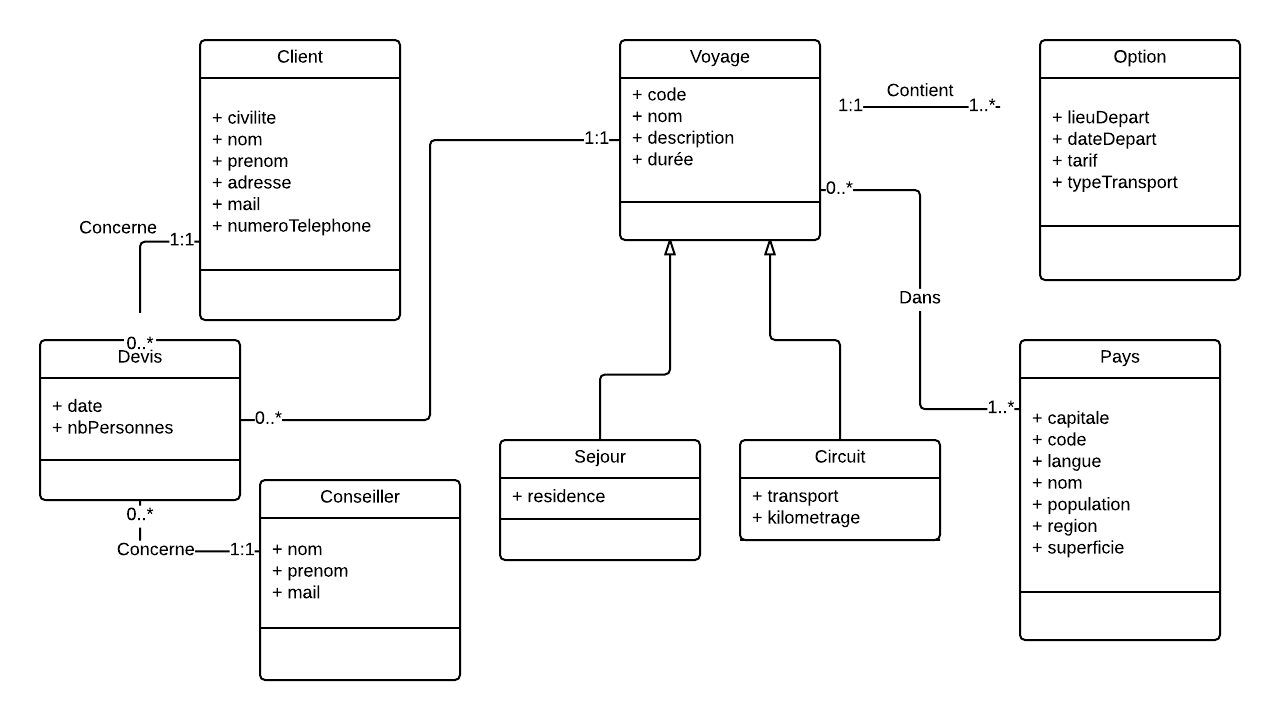
\includegraphics[scale = 0.7]{./Pictures/ModeleDomaine.png}
\newline
Modèle de domaine
\label{fig:ModeleDomaine}
\end{center}
Ce modèle nous permet de stocker toutes les informations nécessaires au fonctionnement de l'application.

\section{Spécification des IHM}
\subsection{IHM Client fenêtrée}
\subsubsection{Présentation}
Cette IHM est celle qui est destinée aux employés de l'agence de voyage. C'est à partir de là qu'il peuvent gérer le catalogue de voyage et éventuellement les devis et informations renseignées sur les pays. Pour ce TP, nous nous sommes limités à  la gestions des voyages. 
\paragraph{Créateur - Connexion}
La première fenêtre à l'ouverture de l'application est une fenêtre de connexion ou l'employé peut s'identifier grâce à son adresse e-mail. Dans le futur, cette identification pourrait permettre de limiter les accès aux fonctionnalités de l'application suivant les catégories d'employés. Elle se présente sous la forme suivante:
\begin{center}
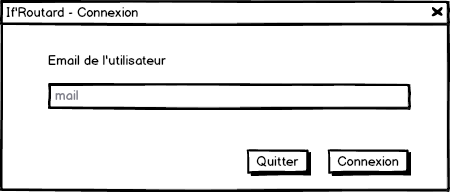
\includegraphics[scale = 0.5]{../Conception_graphique/png_Pour_CR/Createur-00-Connexion.png}
\newline
Créateur - Connexion
\label{fig:Cr-Connexion}
\end{center}
\paragraph{Créateur - Accueil}
Après leur connexion, les employés de l'agence de voyage arrivent sur l'écran d'accueil. À	partir de cette écran, ils peuvent accéder aux différents objets pouvant les intéresser, c'est à dire, les voyages, les devis ou encore les pays (pour une mise à jour des données ou une consultation par exemple). C'est aussi à partir de cette fenêtre qu'ils peuvent se déconnecter de leur compte. Elle se présent sous la forme suivante:
\begin{center}
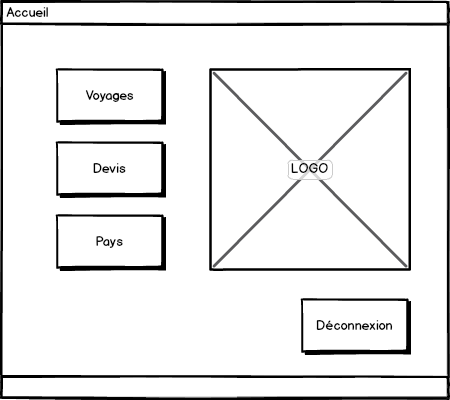
\includegraphics[scale = 0.5]{../Conception_graphique/png_Pour_CR/Createur-10-Accueil.png}
\newline
Créateur - Accueil
\label{fig:Cr-Accueil}
\end{center}

\paragraph{Créateur - Liste Voyages}
À partir de cette fenêtre, les créateurs peuvent rechercher un voyage sur lequel ils souhaitent travailler. Il sélectionnent le voyage qui les intéresse dans la liste et peuvent alors le modifier, le supprimer ou le consulter. Il peuvent aussi créer un nouveau voyage à partir de cette fenêtre. Il peuvent aussi revenir à l'écran d'accueil à partir de cette fenêtre. Elle se présente sous la forme suivante:
\begin{center}
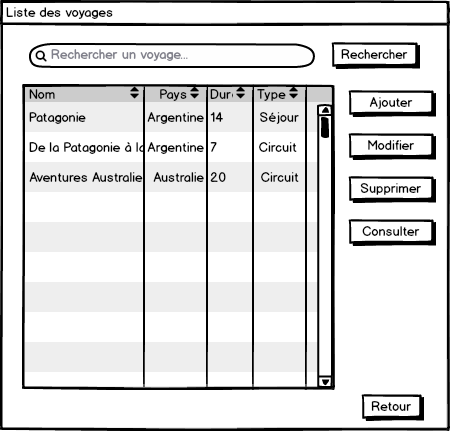
\includegraphics[scale = 0.5]{../Conception_graphique/png_Pour_CR/Createur-20-Liste_Voyages.png}
\newline
Créateur - Liste Voyages
\label{fig:Cr-Liste_Voyage}
\end{center}

\paragraph{Créateur - Fiche Voyage}
Cette fenêtre est celle ou l'employé de l'agence de voyage peut consulter les détails d'un voyage. On peut y accéder à partir de la fenêtre \hyperref[fig:Cr-Liste_Voyage]{Liste Voyage} et les attributs qui la constituent sont différemment accessible selon le choix effectué précédemment. Par exemple, dans le cas d'une consultation ou d'une suppression, aucun des champs ne sera modifiable. Dans le cas d'un ajout, tous les champs seront affichés vide et pour une modification, les champs contiendront les informations du voyage mais seront modifiables. Elle se présente sous la forme suivante:
\begin{center}
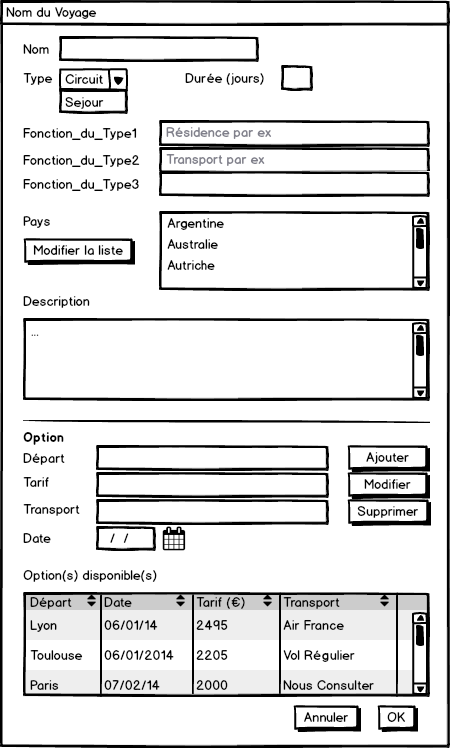
\includegraphics[scale = 0.5]{../Conception_graphique/png_Pour_CR/Createur-30-Fiche_Voyage.png}
\newline
Créateur - Fiche Voyage
\label{fig:Cr-Fiche Voyage}
\end{center}

\paragraph{Créateur - Liste Pays}
Cette fenêtre est utilisée pour ajouter ou modifier plus simplement les pays concernés par un voyage lors de sa création ou de sa modification : elle permet de s'assurer que les pays ajouter sont bien existants dans notre base de donnée et d’éviter les fautes de frappe. Elle se présente sous la forme suivante:
\begin{center}
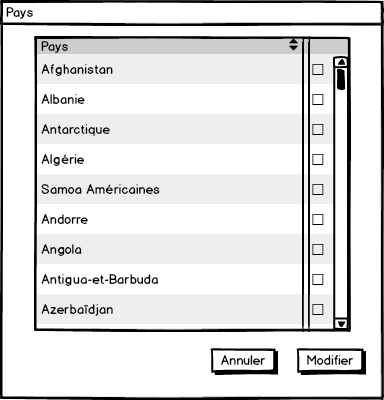
\includegraphics[scale = 0.5]{../Conception_graphique/png_Pour_CR/Createur-40-Liste_Pays.png}
\newline
Créateur - Liste Pays
\label{fig:Cr-Liste Pays}
\end{center}

\subsubsection{ICARs - Client fenêtré}
Cette partie synthétise dans un tableau les ICARs de l'application client fenêtré.\\
\begin{center}
\begin{footnotesize}


\begin{supertabular}{|p{2cm}|p{3cm}|p{3.5cm}|p{2cm}|p{4cm}|}
\hline         
Fenêtre & Intention & Contrôle & Action & Réponse \\ \hline
Créateur - Connexion & Se connecter à l'application & Zone de texte et Bouton "connexion" & Entrée clavier puis click & Accès à la fenêtre Créateur – Accueil   \\ \hline
& Quitter l'application & Bonton \emph{Quitter} & Click & Fermeture de l'application \\ \hline
Créateur – Accueil & Travailler sur les voyages & Bouton \emph{Voyages} & Click & Accès à la fenêtre Créateur – Liste Voyage \\ \hline
 & Se déconnecter & Bouton \emph{Déconnexion} & Click & Accès à la fenêtre Créateur – Connexion \\ \hline
Créateur – Liste Voyage & Rechercher un voyage & Zone de recherche puis bouton \emph{Rechercher} & Entrée clavier puis click & Mise à jour de la liste \\ \hline
 & Trier par Nom/Pays/Durée/Type & Liste des voyages – en tête & Click & Mise à jour de la liste \\ \hline
 & Ajouter / Modifier / Supprimer / Consulter un voyage & Liste et bouton \emph{Ajouter/Modifier/Supprimer/Consulter} & Sélection puis click & Accès à la fenêtre Créateur – Fiche Voyage \\ \hline
 & Revenir à l’écran précédent & Bouton \emph{Retour} & Click & Accès à a fenêtre Créateur – Accueil \\ \hline
Créateur – Fiche Voyage & Modifier le(s) pays concerné(s) par le voyage & Modifier la liste & Click & Ouverture de la  fenêtre Créateur – Liste Pays \\ \hline
 & Ajouter une option & Bouton \emph{Ajouter} & Entrée clavier puis click & Mise à jour de la  liste des options et création \\ \hline
 & Modifier une option & Liste puis zone de texte puis bouton\emph{Modifier} & Sélection puis entrée clavier puis click & Mise à jour de la  liste des options \\ \hline
 & Supprimer une option & Liste et bouton \emph{Supprimer} & Sélection puis click & Mise à jour de la  liste des options \\ \hline
 & Valider les modifications apportées au voyage & Bouton \emph{OK} & Click & Accès à la fenêtre Créateur – Liste Voyage et Création - Modifications \ldots \\ \hline
 & Annuler les modifications & Bouton \emph{Annuler} & Click & Accès à la fenêtre Créateur – Liste Voyage \\ \hline
Créateur – Liste Pays & Trier par Nom & Liste des Pays – en tête & Click & Mise à jour de la liste \\ \hline
 & Modifier le() )pays concerné(s) par le voyage & Sélection puis bouton \emph{Modifier} & Click(s) & Retour à la fenêtre Créateur – Fiche Voyage \\ \hline
 & Annuler les modifications apportées à la liste des pays & Bouton \emph{Annuler} & Click & Retour à la fenêtre Créateur – Fiche Voyage \\ 
 \hline
\end{supertabular}
\end{footnotesize}
\end{center}

\subsection{IHM - Client Web}
\subsubsection{Présentation}
Cette IHM est celle destinée aux clients de l'agence; c'est à partir de là qu'ils peuvent consulter le catalogue des voyages et établir un devis correspondant à leurs besoins.
\paragraph{Web - Accueil}
Cette fenêtre est la page d'accueil du site. À partir de cette page, le client peut s'identifier grâce à son adresse e-mail pour accéder à la recherche des voyages ou choisir de créer son compte client. Elle se présente sous la forme suivante: 
\begin{center}
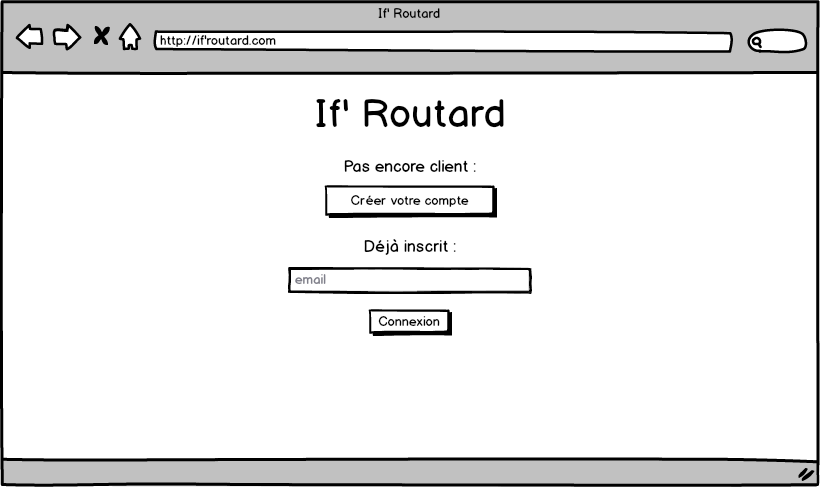
\includegraphics[scale = 0.4]{../Conception_graphique/png_Pour_CR/Web-00-Accueil.png}
\newline
Web - Accueil
\label{fig:Web-Accueil}
\end{center}

\paragraph{Web - Création Compte}
Dans cette fenêtre, le nouveau client doit renseigner les informations qui permettront de créer le nouveau client dans la base de donnée. À la suite de cette création, un e-mail lui est envoyé puis confirmer ou non la création du compte client. Elle se présente sous la forme suivante:
\begin{center}
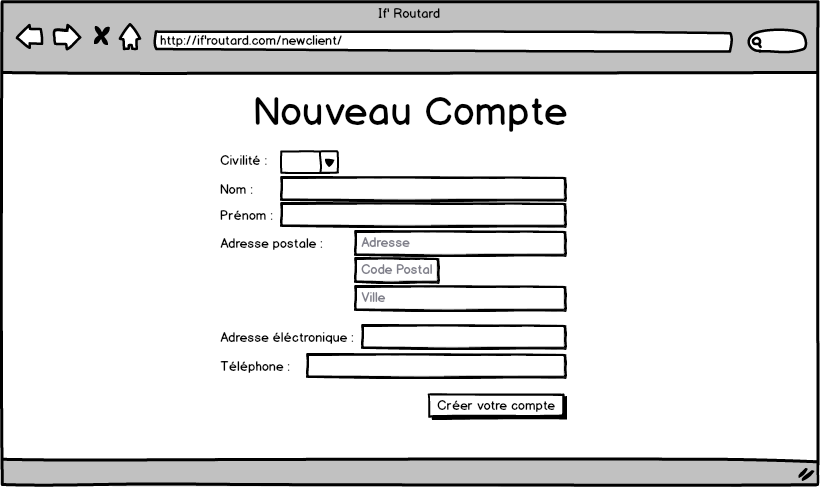
\includegraphics[scale = 0.4]{../Conception_graphique/png_Pour_CR/Web-10-Creation_Compte.png}
\newline
Web - Création Compte
\label{fig:Creation-Compte}
\end{center}

\paragraph{Web - Recherche}
Une fois identifié, le client accède à la page de recherche à partir de laquelle il peut rechercher un voyage par pays ou par type, mais aussi se déconnecter. Elle se présente sous la forme suivante:
\begin{center}
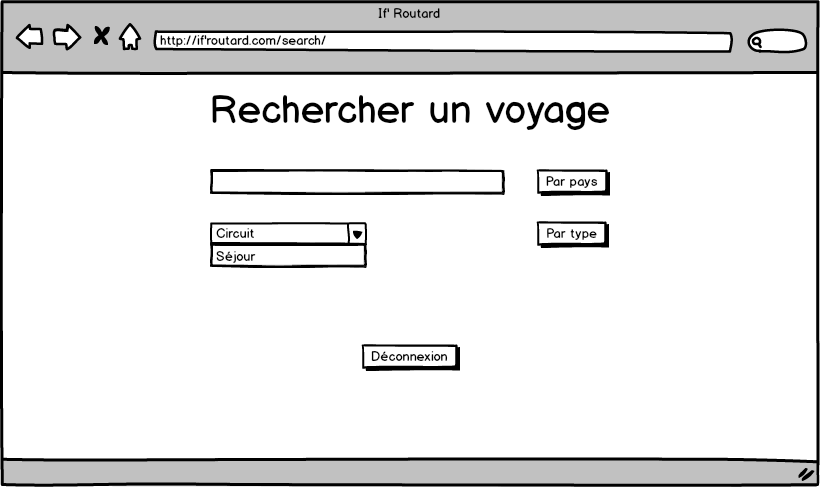
\includegraphics[scale = 0.4]{../Conception_graphique/png_Pour_CR/Web-20-Recherche.png}
\newline
Web - Recherche
\label{fig:Recherche}
\end{center}

\paragraph{Web - Résultats}
Après la recherche, les résultats sont affichés dans une liste sur une nouvelle page. À partir de cette page, le client peut choisir d'obtenir plus de détails sur les voyages affichés (il n'y a que le nom, le pays, la durée et le type dans la liste). Il peut aussi revenir à 'écran précédent pour effectuer une nouvelle recherche. Elle se présente sous la forme suivante:
\begin{center}
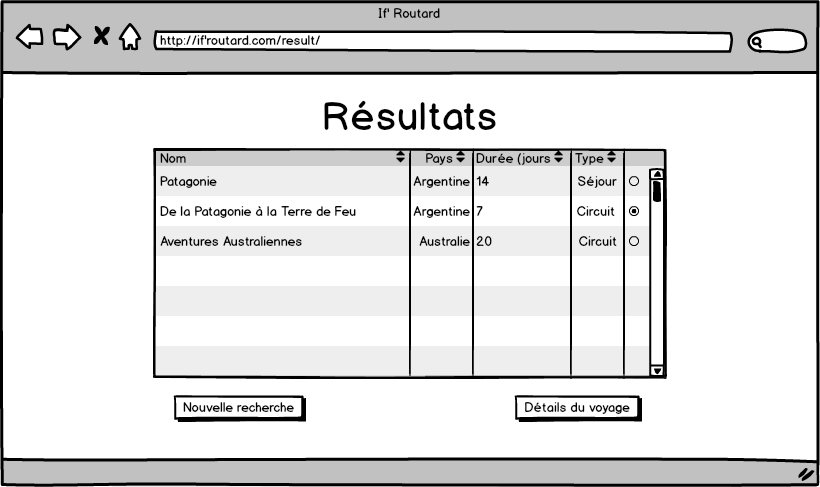
\includegraphics[scale = 0.4]{../Conception_graphique/png_Pour_CR/Web-30-Resultats.png}
\newline
Web - Résultats
\label{fig:Resultat}
\end{center}

\paragraph{Web - Voyage}
Cette page est affichée lorsque le client demande des détails sur l'un des voyages de la liste de résultats. Elle contient toutes les informations concernant le voyage ainsi que la liste des options de départ correspondantes. Sur cette page, en choisissant une option et un nombre de participant, le client peut générer un devis qui sera affiché et envoyé par e-mail. Il peut aussi revenir à la liste de résultats qu'il a obtenu précédemment. Elle se présente sous la forme suivante:
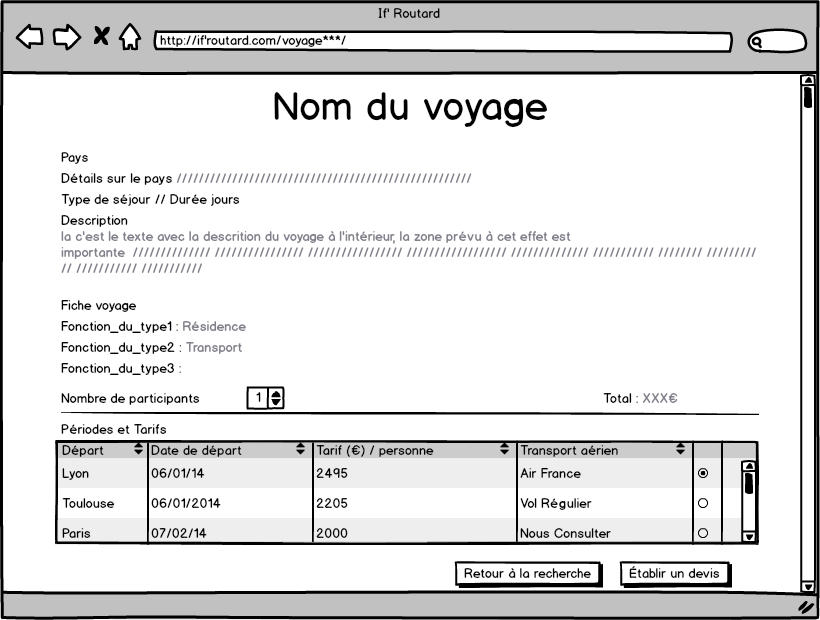
\includegraphics[scale = 0.4]{../Conception_graphique/png_Pour_CR/Web-40-Voyage.png}
\newline
Web - Voyage
\label{fig:Voyage}
\end{center}

\subsubsection{ICARs}

\section{Services}


\end{document}